\scanpage{120}
\diagram{\begin{tikzcd}[ampersand replacement=\&,column sep=huge]
(\text{Préschémas quasi-séparés})
 \arrow[r,"\overline\alpha"]
 \arrow[rr,bend left=28,"\overline\sigma"]
\&\begin{gathered}\operatorname{Ind}(\mathrm{Cons\ cpt})\ \text{flasques}\\\text{''}\\(\mathrm{Cons})\end{gathered}
 \arrow[r,"\overline\beta","{\text{\unsure{submersif}}}"']
\&\left(\begin{gathered}\text{schémas loc. cpts}\\\text{réduits}\end{gathered}\right)
 \arrow[l,bend left=30,"{\overline\beta'\quad\text{pl. fid}}"']
 \arrow[ll,bend left=42,"{\overline\sigma'\quad\text{pl. fid}}"']
\end{tikzcd}}

\diagram{\begin{tikzcd}[ampersand replacement=\&,column sep=small,row sep=large]
\operatorname{Hom}(\overline K,\overline\beta\overline{\mathcal Y})
\&\simeq\operatorname{Hom}(\overline\beta'(K),\overline{\mathcal Y})\arrow[dr,bend right=25]
\&\simeq\varprojlim_{\unsure{\lambda|\rho}}\varinjlim_{\unsure{\mu|\beta}}\operatorname{Hom}(\overline K_\lambda,\beta\overline{\mathcal Y}_\mu))
\\
\&\&\simeq\varprojlim_\lambda\varinjlim_\mu\operatorname{Hom}(\beta'(\overline K_\lambda),\overline{\mathcal Y}_\mu)
\end{tikzcd}}

\deleted{\[
\operatorname{Hom}(\overline K,\unsure{\overline\sigma|\overline\beta}(X))\simeq
\]}
\figure{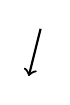
\begin{tikzpicture}[x=1cm,y=1cm]\draw[->,thick](.15,.6)--(0,0);\end{tikzpicture}}
\inserted{\[
\begin{aligned}
\operatorname{Hom}(K,\overline\sigma(X))&\simeq\operatorname{Hom}(\overline\sigma'K,X)\\
&\simeq\varprojlim_\lambda\varinjlim_\mu\operatorname{Hom}(K_\lambda,\sigma(X_\mu))\\
&\simeq\varprojlim_\lambda\varinjlim_\mu\operatorname{Hom}(\sigma'K_\lambda,\deleted{\unsure{\alpha}}X_\mu)
\end{aligned}
\]}

\diagram{\begin{tikzcd}[ampersand replacement=\&]
(\mathrm{Cons})\arrow[r,"{\text{pl. fid}}"]\&\underrightarrow{\operatorname{Hom}}((\mathrm{Cons\ cpt})^\circ,(\unsure{\mathrm{Cons}|\mathrm{Ens}}))
\end{tikzcd}}
\margin{119}
